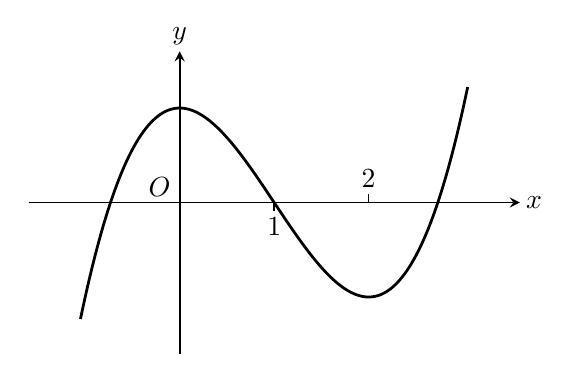
\begin{tikzpicture}[x=1.2cm,y=0.6cm,line width=.6pt,>=stealth]
\draw[->] (-1.6,0)--(3.6,0) node[right,inner sep=0pt,xshift=2pt] {$x$};
\draw[->] (0,-3.2)--(0,3.2) node[above,inner sep=0pt,yshift=2pt] {$y$};
\node[above left,inner sep=0pt,xshift=-3pt,yshift=2pt] at (0,0) {$O$};
\draw (1,0)--++(0,-3pt);
\draw (2,0)--++(0,3pt);
\node[below,inner sep=0pt,yshift=-5pt] at (1,0) {$1$};
\node[above,inner sep=0pt,yshift=5pt] at (2,0) {$2$};
\draw[line width=1pt,domain=-1.05:3.05,samples=160] plot (\x,{\x*\x*\x-3*\x*\x+2});
\end{tikzpicture}
